\documentclass{standalone}

\usepackage{tikz}
\usetikzlibrary{arrows.meta}

\begin{document}
	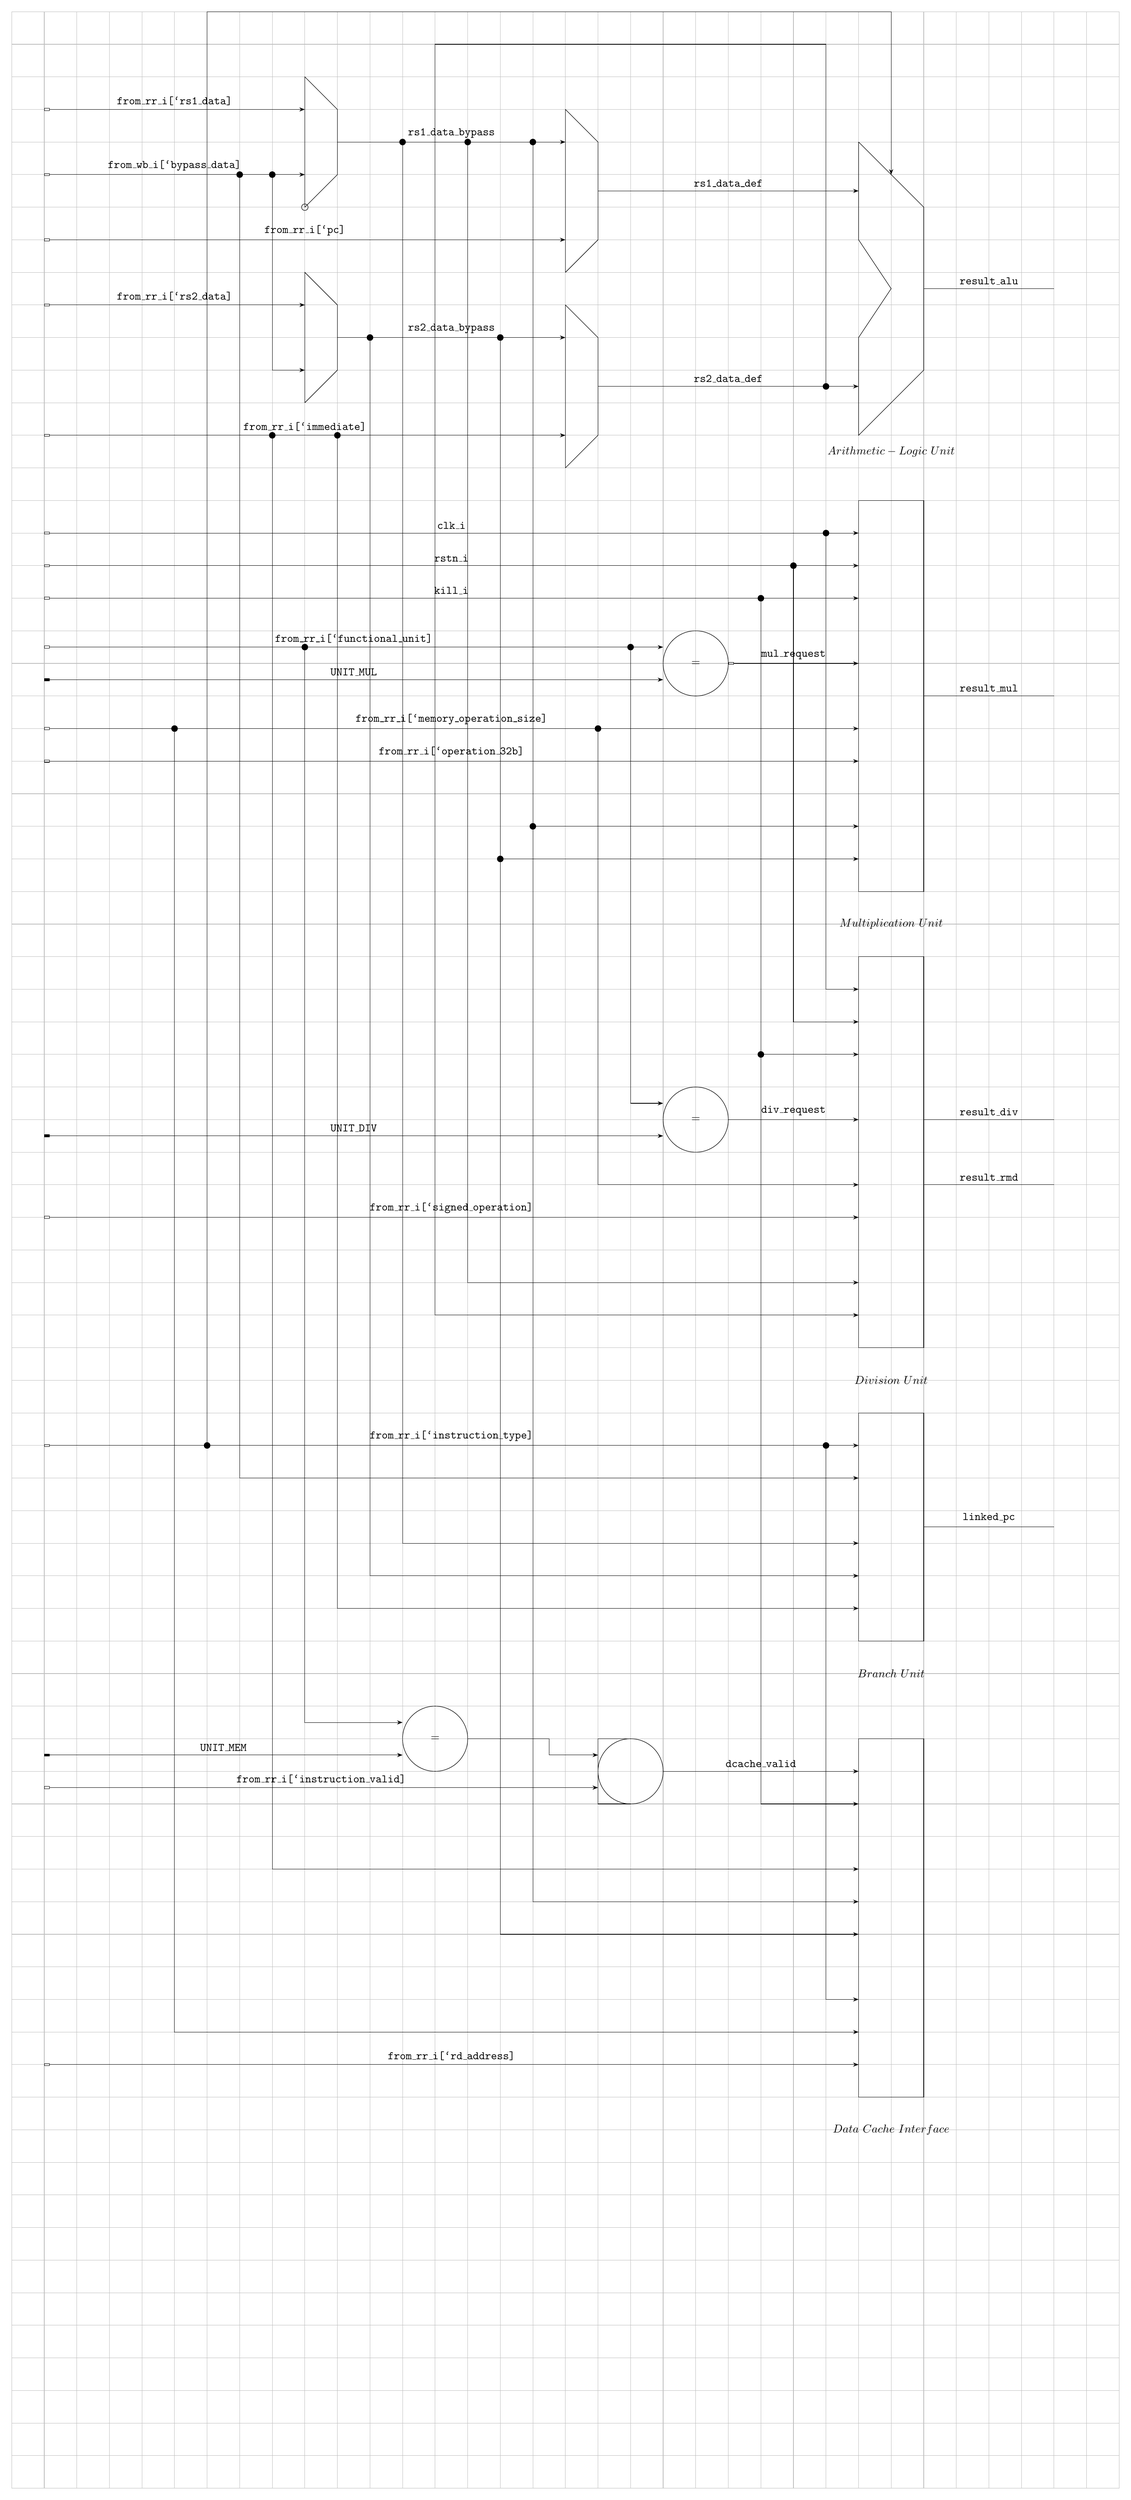
\begin{tikzpicture}
		\draw[lightgray] (-9, -70 ) grid (25, 6);
		\draw (0, 0) circle [radius=0.1];
		
		% Sub-Modules
		% Arithmetic-Logic Unit
		\draw (17, 2) -- (17, -1) -- (18, -2.5) -- (17, -4) -- (17, -7) -- (19, -5) -- (19, 0) -- (17, 2);
		
		% Multiplication Unit
		\draw (17, -21) rectangle (19, -9);
		
		% Division Unit
		\draw (17, -35) rectangle (19, -23);
		
		% Branch Unit
		\draw (17, -44) rectangle (19, -37);
		
		% Comparators
		\draw (12, -14) circle [radius=1];
		\draw (12, -28) circle [radius=1]; 
		
		% Sub-Module Labels
		\node at (18, -7.5) {$Arithmetic-Logic\ Unit$};
		\node at (18, -22) {$Multiplication\ Unit$};
		\node at (12, -14) {$=$};
		\node at (12, -28) {$=$};
		\node at (18, -36) {$Division\ Unit$};
		\node at (18, -45) {$Branch\ Unit$};
		
		% Multiplexers
		% rs1_data_bypass
		%\draw (0, -2) -- (0, 2) -- (1, 1) -- (1, -1) -- (0, -2);
		
		\draw (0, 0) -- (0, 4) -- (1, 3) -- (1, 1) -- (0, 0);
		
		% rs2_data_bypass
		\draw (0, -6) -- (0, -2) -- (1, -3) -- (1, -5) -- (0, -6);
		
		% bypass_pc
		\draw (8, -2) -- (8, 3) -- (9, 2) -- (9, -1) -- (8, -2);
		
		% bypass_immediate
		\draw (8, -8) -- (8, -3) -- (9, -4) -- (9, -7) -- (8, -8);
		
		% Signals
		% from_rr_i[`rs1_data]
		\draw [{Rectangle[open]}-Stealth] (-8, 3) -- (0, 3) node [midway, above] {\texttt{from\_rr\_i[`rs1\_data]}};
		
		% from_wb_i[63:0]
		\draw [{Rectangle[open]}-Stealth] (-8, 1) -- (0, 1) node [midway, above] {\texttt{from\_wb\_i[`bypass\_data]}};
		
		% rs1_data_bypass
		\draw [-Stealth] (1, 2) -- (8, 2) node [midway, above] {\texttt{rs1\_data\_bypass}};

		% from_rr_i[`rs2_data]
		\draw [{Rectangle[open]}-Stealth] (-8, -3) -- (0, -3) node [midway, above] {\texttt{from\_rr\_i[`rs2\_data]}};
		
		% from_wb_i[63:0]
		\draw [-Stealth] (-1, 1) -- (-1, -5) -- (0, -5);
		
		% rs2_data_bypass
		\draw [-Stealth] (1, -4) -- (8, -4) node [midway, above] {\texttt{rs2\_data\_bypass}};
		
		% from_rr_i[`pc]
		\draw [{Rectangle[open]}-Stealth] (-8, -1) -- (8, -1) node [midway, above] {\texttt{from\_rr\_i[`pc]}};
		
		% from_rr_i[`immediate]
		\draw [{Rectangle[open]}-Stealth] (-8, -7) -- (8, -7) node [midway, above] {\texttt{from\_rr\_i[`immediate]}};
		
		% Arithmetic-Logic Unit Signals
		\draw [-Stealth] (-3, -38) -- (-3, 6) -- (18, 6) -- (18, 1);
		
		% rs1_data_def
		\draw [-Stealth] (9, 0.5) -- (17, 0.5) node [midway, above] {\texttt{rs1\_data\_def}};
		
		% rs2_data_def
		\draw [-Stealth] (9, -5.5) -- (17, -5.5) node [midway, above] {\texttt{rs2\_data\_def}};
		
		% Multiplier clk_i
		\draw [{Rectangle[open]}-Stealth] (-8, -10) -- (17, -10) node [midway, above] {\texttt{clk\_i}};
		
		% Multiplier rstn_i
		\draw [{Rectangle[open]}-Stealth] (-8, -11) -- (17, -11) node [midway, above] {\texttt{rstn\_i}};
		
		% Multiplier kill_i
		\draw [{Rectangle[open]}-Stealth] (-8, -12) -- (17, -12) node [midway, above] {\texttt{kill\_i}};
		
		% from_rr_i[`functional_unit]
		\draw [{Rectangle[open]}-Stealth] (-8, -13.5) -- (11, -13.5) node [midway, above] {\texttt{from\_rr\_i[`functional\_unit]}};
		
		% from_rr_i[`functional_unit]
		\draw [Rectangle-Stealth] (-8, -14.5) -- (11, -14.5) node [midway, above] {\texttt{UNIT\_MUL}};
		
		% Multiplier mul_request
		\draw [{Rectangle[open]}-Stealth] (13, -14) -- (17, -14) node [midway, above] {\texttt{mul\_request}};
		
		% Multiplier mul_request
		\draw [{Rectangle[open]}-Stealth] (-8, -16) -- (17, -16) node [midway, above] {\texttt{from\_rr\_i[`memory\_operation\_size]}};
		
		% Multiplier mul_request
		\draw [{Rectangle[open]}-Stealth] (-8, -17) -- (17, -17) node [midway, above] {\texttt{from\_rr\_i[`operation\_32b]}};
		
		% Multiplier rs1_data_bypass
		\draw [-Stealth] (7, 2) -- (7, -19) -- (17, -19);
		
		% Multiplier rs2_data_bypass
		\draw [-Stealth] (6, -4) -- (6, -20) -- (17, -20);
		
		% Division Unit's clk_i
		\draw [-Stealth] (16, -10) -- (16, -24) -- (17, -24);
		
		% Division Unit's rstn_i
		\draw [-Stealth] (15, -11) -- (15, -25) -- (17, -25);
		
		% Division Unit's kill_i
		\draw [-Stealth] (14, -12) -- (14, -26) -- (17, -26);
		
		% Division Unit's Functional Unit
		\draw [-Stealth] (10, -13.5) -- (10, -27.5) -- (11, -27.5);
		
		% Division Unit's Operation
		\draw [Rectangle-Stealth] (-8, -28.5) -- (11, -28.5) node [midway, above] {\texttt{UNIT\_DIV}};
		
		\draw [-Stealth] (13, -28) -- (17, -28) node [midway, above] {\texttt{div\_request}};
		
		\draw [-Stealth] (9, -16) -- (9, -30) -- (17, -30);
		\draw [{Rectangle[open]}-Stealth] (-8, -31) -- (17, -31) node [midway, above] {\texttt{from\_rr\_i[`signed\_operation]}};
		
		\draw [-Stealth] (5, 2) -- (5, -33) -- (17, -33);
		\draw [-Stealth] (16, -5.5) -- (16, 5) -- (4, 5) -- (4, -34) -- (17, -34);
		
		% Branch Unit
		\draw [{Rectangle[open]}-Stealth] (-8, -38) -- (17, -38) node [midway, above] {\texttt{from\_rr\_i[`instruction\_type]}};
		
		\draw [-Stealth] (-2, 1) -- (-2, -39) -- (17, -39);
		\draw [-Stealth] (3, 2) -- (3, -41) -- (17, -41);
		\draw [-Stealth] (2, -4) -- (2, -42) -- (17, -42);
		\draw [-Stealth] (1, -7) -- (1, -43) -- (17, -43);
		
		% ----- Arithmetic-Logic Unit Signals ----- %
		\draw (19, -2.5) -- (23, -2.5) node [midway, above] {\texttt{result\_alu}};
		
		% ----- Multiplication Unit Signals ----- %
		\draw (19, -15) -- (23, -15) node [midway, above] {\texttt{result\_mul}};
		
		% ----- Division Unit Signals ----- %
		\draw (19, -28) -- (23, -28) node [midway, above] {\texttt{result\_div}};
		
		\draw (19, -30) -- (23, -30) node [midway, above] {\texttt{result\_rmd}};
		
		% ----- Branch Unit Signals ----- %
		\draw (19, -40.5) -- (23, -40.5) node [midway, above] {\texttt{linked\_pc}};
		
		% ----- Data Cache Interface ----- %
		% Data Cache Interface
		\draw (17, -58) rectangle (19, -47);
		\node at (18, -59) {$Data\ Cache\ Interface$};
		\draw (4, -47) circle [radius=1];
		\node at (4, -47) {$=$};
		\draw [-Stealth] (11, -48) -- (17, -48) node [midway, above] {\texttt{dcache\_valid}};
		\fill (0, -13.5) circle [radius=0.1];
		\draw [-Stealth] (0, -13.5) -- (0, -46.5) -- (3, -46.5);
		\draw [Rectangle-Stealth] (-8, -47.5) -- (3, -47.5) node [midway, above] {\texttt{UNIT\_MEM}};
		\draw [-Stealth] (5, -47) -- (7.5, -47) -- (7.5, -47.5) -- (9, -47.5);
		\draw [{Rectangle[open]}-Stealth] (-8, -48.5) -- (9, -48.5) node [midway, above] {\texttt{from\_rr\_i[`instruction\_valid]}};
		\fill (14, -26) circle (0.1);
		\draw [-Stealth] (14, -26) -- (14, -49) -- (17, -49);
		\fill (-1, -7) circle (0.1);
		\draw [-Stealth] (-1, -7) -- (-1, -51) -- (17, -51);
		\fill (7, -19) circle (0.1);
		\draw [-Stealth] (7, -19) -- (7, -52) -- (17, -52);
		\fill (6, -20) circle (0.1);
		\draw [-Stealth] (6, -20) -- (6, -53) -- (17, -53);
		\fill (16, -38) circle (0.1);
		\draw [-Stealth] (16, -38) -- (16, -55) -- (17, -55);
		\fill (-4, -16) circle (0.1);
		\draw [-Stealth] (-4, -16) -- (-4, -56) -- (17, -56);
		\draw [{Rectangle[open]}-Stealth] (-8, -57) -- (17, -57) node [midway, above] {\texttt{from\_rr\_i[`rd\_address]}};
		
		% AND Gate
		\begin{scope}
			\draw (10, -47) -- (9, -47) -- (9, -49) -- (10, -49);
			\draw (10, -48) circle (1);
		\end{scope}
		
		% Connection Nodes
		\fill (-1, 1) circle [radius=0.1];
		\fill (7, 2) circle [radius=0.1];
		\fill (6, -4) circle [radius=0.1];
		\fill (16, -10) circle [radius=0.1];
		\fill (15, -11) circle [radius=0.1];
		\fill (14, -12) circle [radius=0.1];
		\fill (10, -13.5) circle [radius=0.1];
		\fill (9, -16) circle [radius=0.1];
		\fill (5, 2) circle [radius=0.1];
		\fill (16, -5.5) circle [radius=0.1];
		\fill (-2, 1) circle [radius=0.1];
		\fill (3, 2) circle [radius=0.1];
		\fill (2, -4) circle [radius=0.1];
		\fill (1, -7) circle [radius=0.1];
		\fill (-3, -38) circle [radius=0.1];
		
		
	\end{tikzpicture}
\end{document}